\documentclass{LibHP20b}

\title{LibHP20b:
A Fully Functional Library for HP20b Calculator Development}
\author{JeanHeyd Meneide}
\date{March 2012}

\begin{document}

\newcommand{\HP}[1][libhp]{\textsc{#1}20b}
\newcommand{\LCD}{\textsc{lcd}}
\newcommand{\RPN}{\textsc{rpn}}
\newcommand{\Sev}{\textsc{s}7}
\newcommand{\Col}[2]{{\color{#1} #2}}
\newcommand{\CWord}[1]{\texttt{#1}}
\newcommand{\CKey}[1]{{\color{blue} \texttt{#1}}}
\newcommand{\CMem}[2]{{\color{blue} \texttt{#1}.}{\color{salmonpink} \texttt{#2}}}
\newcommand{\CPMem}[2]{{\color{blue} \texttt{#1}->}{\color{salmonpink} \texttt{#2}}}
\newcommand{\CFun}[1]{{\color{funccolor} \texttt{#1}}}
\newcommand{\HPButton}[1]{{\color{buttoncolor} \texttt{[ #1 ]}}}
\maketitle

\begin{abstract}

Embedded development is an intricate problem in which one must attempt to create a fully functional machine in as little space (volatile and stored memory) and consume as little time (fast algorithms) as possible, while also with as little developmental feedback (obscure / scarce / cryptic debugging) as possible.
Adding calculator development as the goal of an embedded project sprinkles another layer of challenge; tiny programming routines that need to be memory efficient and fast must also be accurate to the degree of representation allowed by the calculator.
I present \HP, a library for the \HP[hp] Calculator with modular pieces that can be used in other high-precision calculators for embedded development. It features common functions for accessing every part of the liquid crystal display (\LCD) and keyboard, a variable-precision floating-point number sub-library that is accurate to any degree of compile-time specified digits (currently preset to 12), and a few well-organized structures and functions for the \HP[hp] itself (\LCD{} Alignment, 6 x 43 Matrix access,  keyboard state storage, and more).

\end{abstract}

\section{Introduction}
Designed by Hewlett Packard with extra functionalities such as interest/year, permutation, and more~\cite{hp20bmanual}, the \HP[hp] (or just \HP[]) is a rather powerful but small calculator. However, the calculator's firmware was deep-shredded by Professor Stephen A. Edwards and TA Yoonji Shin, leaving it a completely blank JTaggable Development Platform.

The task was to rebuild basic calculator functions and allow you - the reader - to be able to pick up the calculator and perform basic arithmetic (+, -, $\times$, $\div$) in Reverse Polish Notation (\RPN{}) ~\cite{rpninfo}. The User Guide \ref{sec:tutorial} will walk you through using the reprogrammed \textsc{segment 7} (\Sev) and Matrix LCD Display. 

\section{User Guide}
\label{sec:tutorial}
The \HP[hp] Calculator works in a permanent \RPN mode. This means that you enter a series of numbers first, before pressing an operation key (+, -, $\times$, $\div$) to perform an operation.\\
In order to start the \HP[], turn the calculator on. The first number in any \RPN{} calculation is special: it begins the \RPN{} chaining mode. As you enter numbers, the \LCD{} Matrix display will show the count of Numbers currently registered in your \RPN{} chain. When it is 0 (while the \RPN{} chain is still beginning), you will be unable to perform operations until you press the \texttt{input} button, and commit the current number you are editing to the stack. You are still able to perform \emph{in-place} operations, however, such as \texttt{$\frac{1}{x}$} or x$^{2}$. Pressing an in-place operation will modify the number currently displayed on your screen.\\
When you are ready to begin doing operations, hit \HPButton{INPUT}. This will start your \RPN{} chain, storing the number you were working on previously at the back of a chain of numbers. You can now perform any operation you would like. Pressing an operation will perform that operation and commit it to the number underneath the one you are editing. If you would like to reset the whole chain and clear all numbers, simply press \HPButton{Shift}\HPButton{Reset}. Here are some example sequence of commands from the beginning of the \RPN{} chain:\\
\begin{quote}
\center
( Example 1 - adding 0 to the chain )\\
13 \HPButton{INPUT} \HPButton{+}\\
Result: 13\\
( Example 2 - multiplying 0 into the chain )\\
13 \HPButton{INPUT} \HPButton{$\times$}\\
Result: 0
\end{quote}

Both of these examples show that when you increment your \RPN{} chain, you get a fresh, blank 0 to work with. Pressing the operation key directly after performing an operation will perform an operation with the last number you entered and zero. If you try the following:\\
\begin{quote}
\center
( Example 3 - Dividing by Zero )\\
13 \HPButton{INPUT} \HPButton{$\div$}\\
Result: ERROR\\
\end{quote}
The calculator will throw a division by zero error, and reset your \RPN{} chain's current and last number to 0 before decreasing the \RPN{} chain's size by one. This will put you back to the number that was divided into by 0. You can then start typing out numbers on the stack once more. The calculator will throw errors for Overflow and Underflow as well, so be careful of multiply two really huge numbers or dividing a really small number by a really huge number.\\
That covers all you will need to know about the \HP[]. You can make bigger \RPN{} chains for more complex calculations:\\
\begin{quote}
\center
( Example 4 - Averaging a list of numbers )\\
20 \HPButton{INPUT} 25 \HPButton{INPUT} 30 \HPButton{INPUT} 25 \HPButton{+}\HPButton{+}\HPButton{+} 4 \HPButton{$\div$}\\
Result: 25\\[3ex]
\end{quote}


\begin{figure}
\centerline{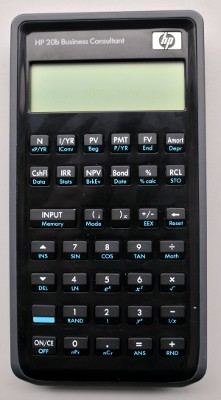
\includegraphics[width=0.3\textwidth]{HP20bCalculator.jpg}}
\caption{The \HP[hp] Calculator}
\label{fig:hp20b}
\end{figure}

\section{Social Implications}

The 20b is lightweight and performs perfectly-accurate variable precision arithmetic on the go, making it ideal for quick calculations, especially on-the-go calculations. Because the Atmel processor consumes so little power, the calculator can actually run for an average of 9 months, making it ideal for usage in a semester of school, especially in places where power is scarce. 

\section{The Platform}

I first learned about hacking the \HP[hp] (\figref{hp20b}) from the \emph{\HP[hp] repurposing project} website~\cite{hp20b-repurposing}. From here, I learned about the JTaggable Development Interface and was further directed to read about the Atmel \textsc{at91sam7l128}, the \LCD{}, and the keyboard.

\subsection{The Processor}

The 20b is little more than a keyboard and \LCD{}, having an Atmel~\textsc{at91sam7l128} (\textsc{sam7l}) processor. The name was birthed from it being a part of Atmel's \textsc{at91}-\\\textsc{sam} series of chips, which are all built around an \textsc{arm} processor core (``\textsc{at}'' is for Atmel;
``\textsc{sam}'' is ``smart \textsc{arm} core''). The \textsc{7l} series of microcontrollers are designed for low power (hence the \textsc{l}), and the final~128 is a reminder that it includes 128K of flash program memory.

The processor natively supports the following C programming language intrinsic types: \emph{\CKey{char} (8 bits, 1 byte), \CKey{short} (16 bits, 2 bytes),} and \emph{\CKey{int} (32 bits, 4 bytes)}. It supports IEEE-754-compatible Single Precision floating point arithmetic (\emph{\CKey{float} (32 bits, 4 bytes)}) and IEEE-754-compatible Double Precision floating point arithmetic (\emph{\CKey{double} (64 bits, 8 bytes)}). These last two data types, however, are lossy binary representations of human-readable-standard base$-10$, meaning that for the precise decimal calculations needed for a calculator, I would need to "roll my own" arbitrary-precision decimal digit library suitable for variable precision digit arithmetic (see \ref{sec:libvpa}).

Figure \ref{fig:at91sam7l} shows a block diagram of the \textsc{sam7l} chip. It looks complicated, but is essentially a single standard processor surrounded by memory and a wide variety of peripherals, most of which remained unused for \HP. The system controller, through software, controls the clock and power supply of each peripheral which can save energy by deactivating unneeded peripherals (be wary: not turning on a peripheral can result in the LCD being blank despite software display data to it or the keyboard becoming unresponsive even though written software routines are working properly).

\begin{figure}
\centerline{\includegraphics[height=0.9\textheight]{AT91SAM7lBlockDiagram.pdf}}
\caption{A block diagram of the AT91SAM7L microcontroller that is at
  the heart of the \HP{hp}}
\label{fig:at91sam7l}
\end{figure}

\pagebreak

\subsection{The LCD Display}

The \LCD{} of the 20b contains 15 \Sev{} digit displays and two negative signs (3 smaller ones for exponential digits and 12 for the regular digits, and one minus sign for each digit group). There are also an amalgamation of indicators for battery life, memory storage, notations, statuses and input states.\\
It is important to note here that while Figure \ref{fig:hp20blcd} shows comma-display capabilities, the calculators we had were not equipped with commas. In either case, \HP{} is programmed to handle them if you happen to have a \HP[] with the newer \LCD{} model while also being compatible with the older model used for development and quality control of the \HP[hp].

\begin{figure}[h]
\centerline{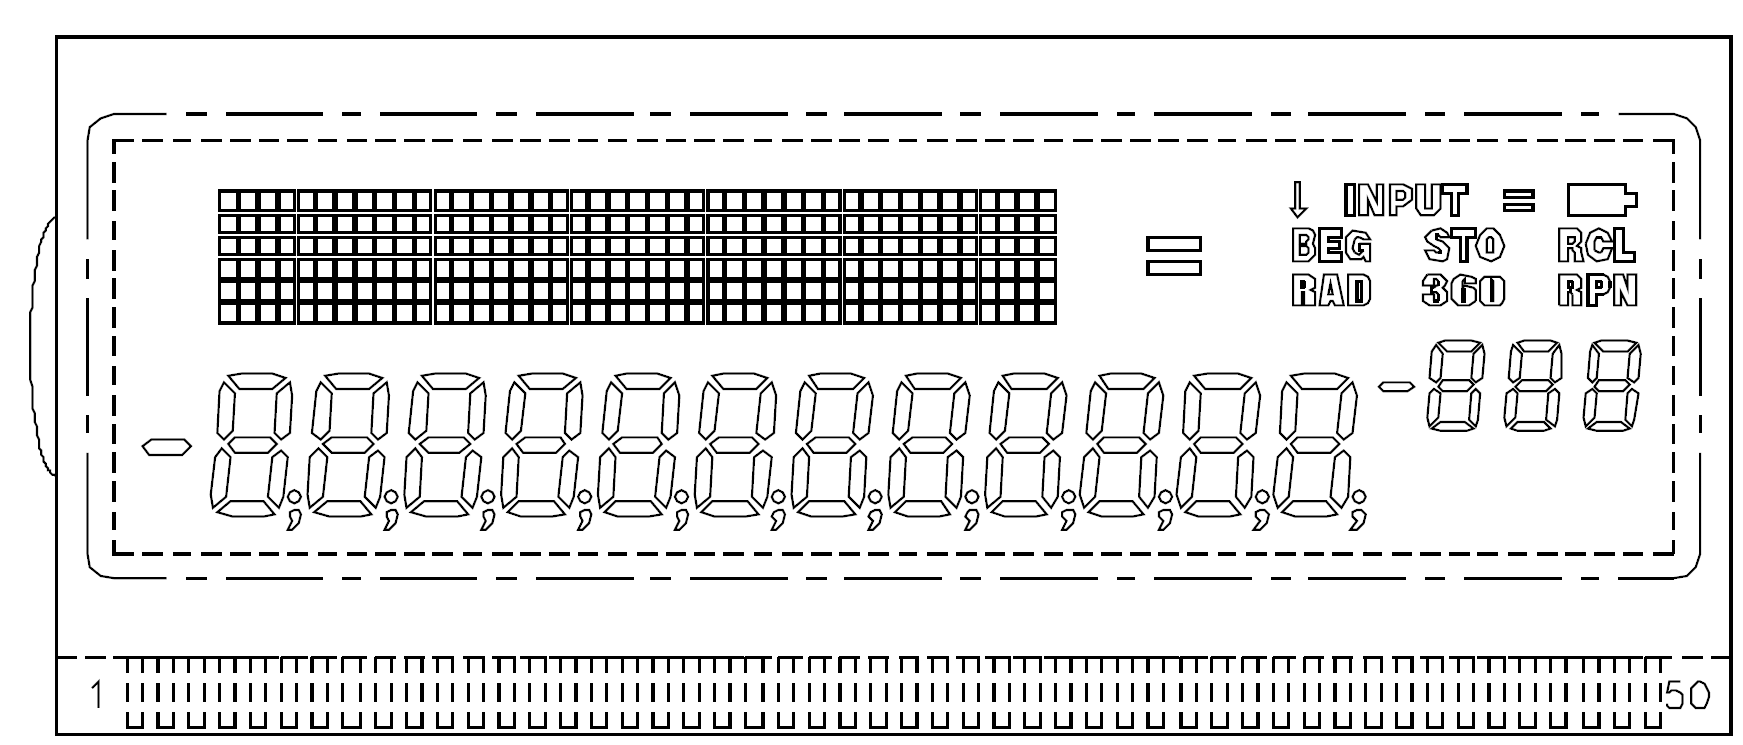
\includegraphics[height=0.4\textwidth]{HP20bLCDLayout.png}}
\caption{The \HP{hp} LCD Screen. It has a 43 x 6 pixel display matrix, various display indicators}
\label{fig:hp20blcd}
\end{figure}

\subsection{The Keyboard}

The \HP[]'s keyboard is a simple cross-wiring of switches and leads  \figref{hp20bkeyboard}. Columns are inputs on the Input/Output (IO) pins, which can be programmed to be at high voltage (\emph{1} or \emph{true} in C terminology) or low voltage (\emph{0} or \emph{false}). Rows (including the special the \HPButton{{ON/CE}} switch/row combination) are outputs, which take on the voltage set by the columns which connect to them. When the switch of a specific column/row cross-wiring is pressed, that row's lead is connected to the column (which is set to 0 during the read), shorting that specific row to 0. One must check for false in order to see if a certain key is down or not. This same logic apples to the \HPButton{ON/CE} key, except it has its own IO pin connected directly to ground, meaning one must simply check the single 'row' for a short.\\
Power is saved when the calculator powers down; rather than have \HPButton{ON/CE} part of the power grid and thus force 12+ peripherals to be constantly drawing power, a single peripheral (arbitrarily determined by the original calculator chip engineers to be I/O pin 10, \figref{hp20bkeyboard}) only needs to test if it has been shorted or not. Only one single peripheral draws power, alongside the required power to keep the programs and memory alive in storage with the Atmel~\textsc{at91sam7l128} in low power mode.

\begin{figure}
\centerline{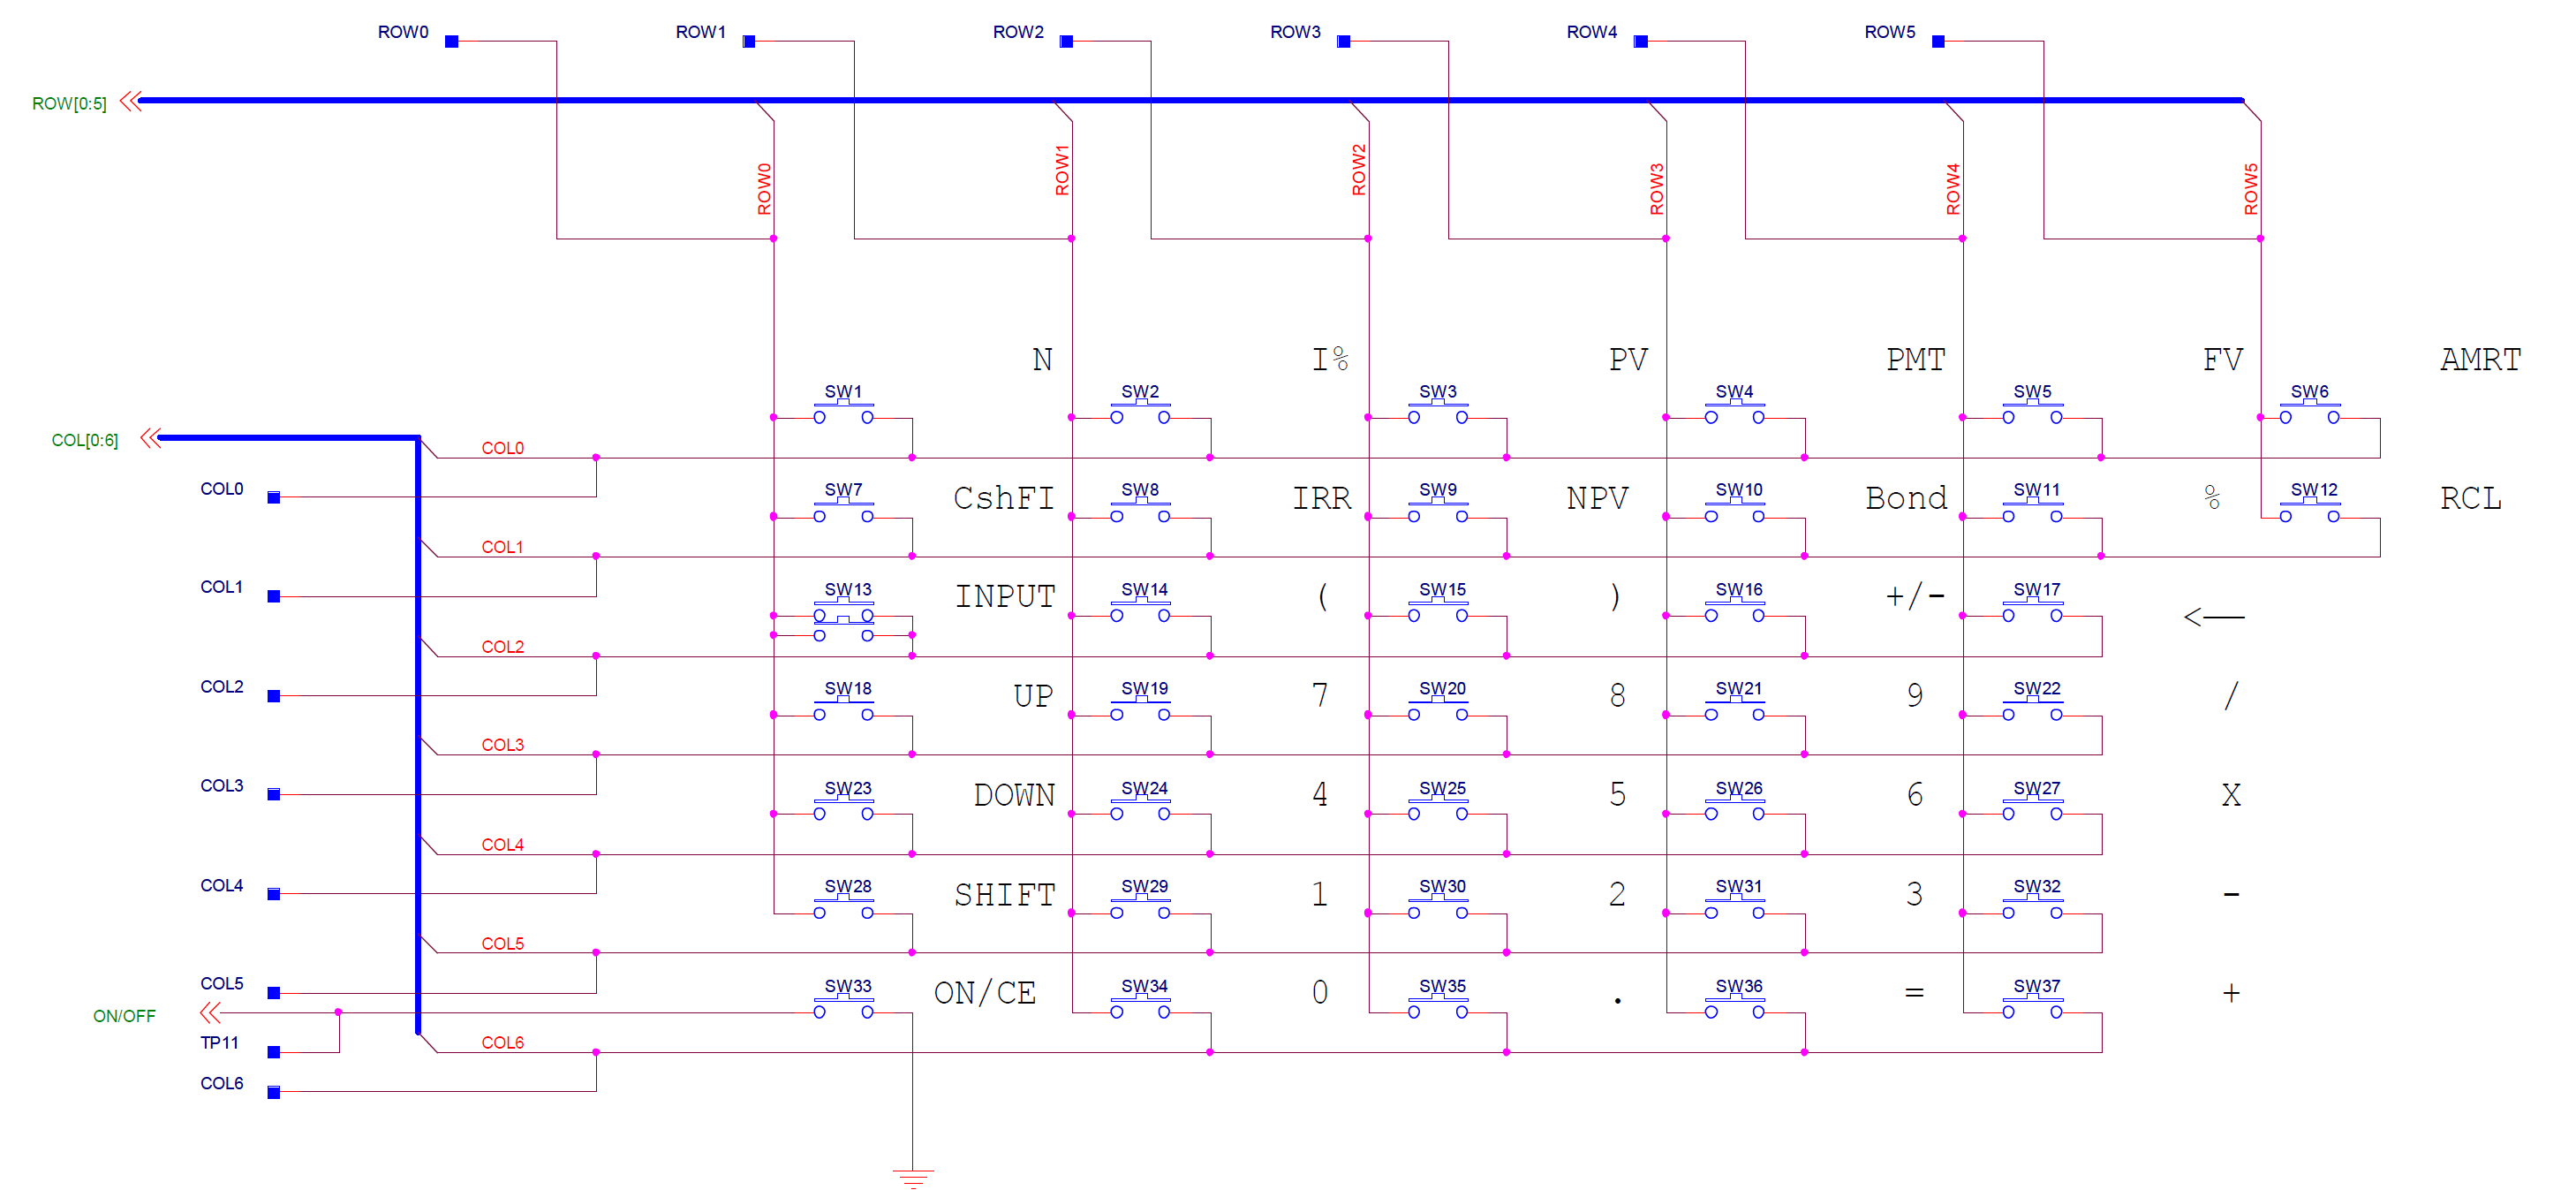
\includegraphics[height=0.4\textheight]{HP20bKeyboardSchematic.png}}
\caption{The \HP[hp] Keyboard wiring schematic. Notice that \HPButton{ON/CE} is on its own output rail to ground (0 volts).}
\label{fig:hp20bkeyboard}
\end{figure}

\section{Software Architecture}

There are three \emph{Subsystems} to \HP{}. Two correspond to core mechanical features of the 20b which are the \LCD{} subsystem and the Keyboard subsystem. The final subsystem is the Watchdog subsystem, which is linked to the internal timer which will universally set a low power state, or even power down the machine after a certain time has passed.\\
Following an \CKey{SDL}-style system \cite{libsdl}, initializing subsystems to use \HP{} is as simple as calling the \CFun{HP20b\_Init} function The \CWord{C language} does not have classes, so functions and structures are named after their functionality and the services they provide. All functions dependent on the LCD subsystem will have LCD in their names, while all functions dependent on the Key subsystem will have Key or Keyboard in their names. There are no functions associated with the watchdog. The source code is available at

\section{Software Details}
\label{sec:softdetails}
Some of the following sections will not have their full source code posted, due to the sheer size of the solutions. You can access the full source code - with hotkey-linked and GUI-friendly build interfaces, debug projects, and more - for both the calculator and various operating systems (see \ref{sec:srccode}). Included in \HP{.tar.gz} are regular desktop-PC project files for Visual Studio (Windows), XCode (Mac OSX), and Eclipse (Windows, Mac OSX, Linux). The projects have been tested and compile on all three platforms (Linux was tested \textsc{via} Fedora 16, KDE), with OpenOCD and a specific embedded compiler (Linaro GCC (Windows and Linux) or CodeSourcery Lite (Mac OSX)).

\subsection{Variable Precision Arithmetic Library}
\label{sec:libvpa}

The Variable Precision Arithmetic Library included with \HP{} is a sturdy implementation of binary-coded decimal, with two tightly-packed \CKey{Nybbles} (\figref{nybbleheader}) compressed into a single byte (4 bits per decimal digit). This was due to three distinct reasons:

\begin{figure}[!htbp]
\begin{Code}
typedef union {
	byte All;
	struct {
		byte Low:4;
		byte High:4;
	};
} Nybble;

typedef union {
	Nybble Cells[7];
	struct {
		union {
			Nybble Mantissa[6];
			struct {
				Nybble MantissaLowest;
				Nybble MantissaPad[4];
				Nybble MantissaHighest;
			};
		};
		union {
			Nybble Info;
			struct {
				byte Exponent:4;
				byte Sign:4;
			};
		};
	};
} Number;
\end{Code}
\caption{The declaration for a single \CKey{Nybble} and a sample declaration of the \CKey{Number} type. A \CKey{Nybble} occupies a single byte (8 bits), and a number occupies a total of 7 bits, 1 less than the size of a \CKey{long long} in \CKey{C}. Because it is essentially an array of type \CKey{unsigned char}, the compiler will automatically use \CFun{memcpy} to copy instances of one number to another. \HP{} includes 3 \CFun{memcpy} implementations for various speeds of copying - see \CWord{Core.h} for details.}
\label{fig:nybbleheader}
\end{figure}

\begin{itemize}
\item 64-bit Integers (\CKey{long} or \CKey{long long} data types in \CWord{C}) are not fully supported, and crashes the firmware of the calculator upon performing basic arithmetic (pointer arithmetic and some bitwise arithmetic is allowed).
\item An unsigned 32-bit integer with another integer to specify a base-10 exponent and a sign bit can only cover up to ten decimal places (maximum of \CWord{4,294,967,296}). This is less than the \HP[hp]'s \LCD{} can handle.
\item The high precision required for a calculator's division would immediately exceed a 32-bit integers attempts at simulating a base-10 number.
\item Error handling for Division by Zero, Overflow, and Underflow are not present within the numeric framework of any built-in data type without reading volatile processor register data.
\end{itemize}

While this wastes about $\frac{1}{6}$ of the possible states represented by 4 bits, it has its advantages in being immediately human-readable and easily translated to and from character strings. Furthermore, multiplication and division by 10 - common operations used by humans - are quick, effortless shifts. It becomes even easier to align two decimal numbers (e.g., 13.1 and 0.54) by simply performing the aforementioned shifts.\\
Complications arise, however, to make this solution work quickly and well with a system based on binary operations. Most hardware - including the Atmel processors - are not prepared to access bits out of an 8-bit aligned boundary, slowing down operations as native pointer arithmetic must be regulated by at least two other bit-masking and bit-shifting variables. Addition and Subtraction with anything other than positive numbers results in having to carefully pad numbers using Nines- and Tens-Complement algorithms, with rigorous signs checking and re-complementing if intermediate results meet certain criterion. Multiplication and division are implemented in accurate, but slow long-hand multiplication and long, decimal-padded division. Furthermore, in order to account for results which may exceed \CKey{Number}'s current maximum digit count, a second format \CKey{HighNumber} with its own routines - which contains about twice as many digits to account for overflow and underflow of answers using the original \CKey{Number} format - is utilized.\\
Because the sign bit is 4 bits, three of those bits can be immediately used to signal overflow, underflow, and division by zero, making checks for irregular conditions from mathematical operations easy.

\subsection{Lab 1: Displaying a Number}
\label{sec:display}

\begin{figure}
\begin{lstlisting}
int IntToString (int value, char* out) {
	int i = 0, j = 0;
	char* p = out;
	if (value == 0) {
		*p++ = '0';
		*p = '\0';
		return 1;
	}
	else if (value < 0) {
		value = -value;
		*p++ = '-';
		++i, ++j;
	}
	for (; value != 0; ++i) {
		*p++ = (value % 10) + 48;
		value /= 10;
	}
	// XOR Swapping Algorithm
	for (--i; j < i; ++j, --i) {
		out[i] ^= out[j];
		out[j] ^= out[i];
		out[i] ^= out[j];
	}
	*p = 0;
	return i + j + (out[0] == '-' ? 0 : 1);
}
\end{lstlisting}
\caption{A general purpose Integer-To-String algorithm for use with the various printing functions. Used for \textsc{lab 1}. Features XOR swapping to align digits correctly, avoid the extra function call, and to save on processor memory usage.}
\label{fig:lab1}
\end{figure}

Taking a basic integer and turning it into a string is a simple task that is used often. The first draft of code put the number's characters directly to the \textsc{s7 lcd}, but this style inhibited flexibility. Figure \ref{fig:lab1} turns what would be a \texttt{main} routine into a rather generic \CFun{ToString} function, allowing the caller to put the results into a \CFun{char} buffer rather than directly to the \LCD{}, achieving portability. All \CFun{ToString} and \CFun{FromString} functions are defined in \CWord{Standard.h} and \CWord{Standard.c}. \figref{lab1} shows integral string creation, but within \CWord{Standard.c} lies functions for \CKey{unsigned integer, float, Decimal}, and \CKey{Number} as well. However, \CKey{Decimal} is an obsolete version of \CKey{Number} and is marked for removal from the library completely; it is only present for educational value.\\
Furthermore, \HP{} features Matrix display capabilities. Various functions are defined for printing strings, integers, and numbers to the Matrix Display; all of these are derived from a single function: \CFun{HP20b\_LCDMatrixGraphic}. You can paint arbitrary pictures (of relatively poor resolution) or use the simple text version of this function to write words to the Matrix Display (\figref{lab1matrix}).

\begin{figure}
\begin{lstlisting}
void HP20b_LCDMatrixGraphic(ullong* graphic) {
	uint c = 0;
	int j = 0, i = 0;
	ullong* lcdmemory = (ullong*)AT91C_SLCDC_MEM;
	// Initial Horizontal memory	
	lcdmemory[6] = (lcdmemory[6] & ~0x7fffffffc0LL) |
					((graphic[0] << 6) & 0x7fffffffc0LL);
	lcdmemory[7] = (lcdmemory[7] & ~0x7fffffffc0LL) |
					((graphic[1] << 6) & 0x7fffffffc0LL);
	lcdmemory[8] = (lcdmemory[8] & ~0x7fffffffc0LL) |
					((graphic[2] << 6) & 0x7fffffffc0LL);
	lcdmemory[9] = (lcdmemory[9] & ~0x7fffffffc0LL) |
					((graphic[3] << 6) & 0x7fffffffc0LL);
	lcdmemory[0] = (lcdmemory[0] & ~0x7fffffffc0LL) |
					((graphic[4] << 6) & 0x7fffffffc0LL);
	lcdmemory[1] = (lcdmemory[1] & ~0x7fffffffc0LL) |
					((graphic[5] << 6) & 0x7fffffffc0LL);
	for (j = 9; j >= 0; j--) {
		c = 0;
		for (i = 0; i < 6; i++) { 
			c = ( c << 1 ); 
			if ((graphic[i] & (LL << (j + 33))) != 0) c++; 
		}
		// We condemn all bits in lsb position < 5 before we
		// take the original graphical data (stored in c) and
		// bitwise OR it to get our final register data.
		lcdmemory[(int)MatrixVerticalShift[j]] =
		(lcdmemory[(int)MatrixVerticalShift[j]] & ~(0x3fLL)) |
			(ullong)c;
	}
}
\end{lstlisting}
\caption{The matrix display function for reading bits from a 64-bit graphical array. The array passed in is 6 \CKey{unsigned long long}'s wide, where the 43 least significant bits of each \CKey{unsigned long long} represents a pixel on the screen. }
\label{fig:lab1matrix}
\end{figure}

\subsection{Lab 2: Scanning the Keyboard}
\label{sec:scanning}
\begin{figure}
\begin{lstlisting}
void HP20b_KeyboardUpdate () {
	int col = 0, row = 0;
	for (col = 0 ; col < HP20B_KEYBOARD_NUMCOLUMNS; col++) {
		HP20b_KeyboardColumnLow(col);
		for (row = 0 ; row < HP20B_KEYBOARD_NUMROWS; row++) {
			if (HP20b_KeyboardRowRead(row) == 0) {
				// If it wasn't already down,
				// The key is "Pressed" (State: Fresh Down)
				if ((HP20b_KeyboardKeys[col][row] & 0x1) == 0)
					HP20b_KeyboardKeys[col][row] |= 0x2;
				else
					HP20b_KeyboardKeys[col][row] &= ~(0x2);
				// Turn off the Release Bit
				HP20b_KeyboardKeys[col][row] &= ~(0x4);
				// Turn on the Down Bit (State: Down)
				HP20b_KeyboardKeys[col][row] |= 0x1;
			}
			else {
				// If already down,
				// The key is "Released" (State: Fresh Up)
				if ((HP20b_KeyboardKeys[col][row] & 0x1) != 0)
					HP20b_KeyboardKeys[col][row] |= 0x4;
				else
					HP20b_KeyboardKeys[col][row] &= ~(0x4);
				// Turn off the Pressed Bit
				HP20b_KeyboardKeys[col][row] &= ~(0x2);
				// Turn off the Down Bit (State: Up)
				HP20b_KeyboardKeys[col][row] &= ~(0x1);
			}
		}
		HP20b_KeyboardColumnHigh(col);
	}
	if (HP20b_KeyboardRowRead(6) == 0) { /* For ON / CE */ }
}
\end{lstlisting}
\label{fig:lab2}
\caption{The code for scanning the keyboard. Note that there is a separate Row-Read for the \textsc{on/ce} button.}
\end{figure}

\begin{figure}
\begin{lstlisting}
typedef enum HP20bKey {
	N, IYR, PV, PMT, FV, Amort,
	CshFl, IRR, NPV, Bond, Percent, RCL,
	Input, OpenParen, CloseParen, Negation, Backspace, BR5C2,
	Up, N7, N8, N9, Divide, BR5C3,
	Down, N4, N5, N6, Multiply, BR5C4,
	Shift, N1, N2, N3, Minus, BR5C5,
	OnClearSurrogate, BR1C6, N0, DecimalPoint, Equals, Plus,
	
	OnClear,

	xPYR, IConv, Beg, PYR, End, Depr,
	Data, Stats, BrkEv, Date, PercentCalc, STO,
	Memory, Mode, ShiftedBR2C2, EEX, Reset, ShiftedBR5C2,
	INS, SIN, COS, TAN, Math, ShiftedBR5C3,
	DEL, LN, eToThex, xSquared, Squareroot, ShiftedBR5C4,
	UnShift, Random, Factorial, yToThex, Inversex, ShiftedBR5C5,
	OffSurrogate, ShiftedBR1C6, nPr, nCr, ANS, Round,
	
	Off
	
} HP20bKeys;
\end{lstlisting}
\label{fig:lab2keyconstants}
\caption{The various key constants representing the shifted and unshifted keys of the 20b.}
\end{figure}

Keyboard scanning was finished rather quickly, having taken a lesson from how an Xbox 360 Controller stores and retrieves its button and controller values~\cite{xbox360}.
While a state-saving system in order to do Key-Down, -Release, -Held, and -Up testing would have been a bit more robust, that would rely too heavily on an update function being called with determined regular frequency. Instead, I stored the individual key's statuses in 4 bits of an array that corresponded to each key. The whole array is then updated all at once, when the user calls the \CFun{HP20b\_KeyboardUpdate} function (\figref{lab2}). After this, the user can then call \CFun{HP20b\_Key...}, where "\CWord{...}" can be any state of \CFun{Down, Up, Released}, or \CFun{Held}. You can also append the word \CFun{Live} before the state to form a function that gets the precise current state of a certain key (e.g. \CFun{HP20b\_KeyLiveDown(Backspace)}), rather than the last value stored from the Update function. There are constants which make it easy to access keys by name within code rather than by a number; for key constants defined in the code, \figref{lab2keyconstants}.\\

Understanding how \textsc{on/ce} button worked allowed me to use it as the clear button. The internal tracking of the first pressed key from function \CFun{int HP20b\_FirstKey} and the uniqueness test specifically for whether or not it was not just the same key pressed twice from \CFun{bool HP20b\_FirstKeyIsUnique)} allowed the \LCD{} to be updated only for a unique first key. Once the key was pressed, it was displayed to the Matrix Display to ensure that the function \CFun{HP20b\_KeyCode} produced the correct keycode; all keys, including \textsc{on/ce} and shifted keys, displayed their correct keycodes.

\subsection{Lab 3: Entering and Displaying Numbers}
\label{sec:entering}

\begin{figure}
\begin{lstlisting}
#define NUMBERSTACKMAX 25
#define S7Size 15
#define MatrixSize 20

struct HP20b_Calculator {
	uint CPUSpeed;
	/* Union booleans for initialized system */
	union {
		byte Status;
		union { struct {
				bool Entering:1;
				bool Postfix:1;
				bool AfterNum:1;
				bool Shifted:1;
				byte DelayedOperation:4;
		};};
	};
	/* Union booleans for aligntment, etc. */
	int ResultStackIndex;
	int OpStackIndex;
	union {
		char Op;
		char OpStack[NUMBERSTACKMAX];
	};
	union {
		Number Result;
		Number ResultStack[NUMBERSTACKMAX];
	};
	char S7[S7Size];
	char Matrix[MatrixSize];
} HP20b;
\end{lstlisting}
\label{fig:hp20bstruct}
\caption{The pertinent pieces of the \HP[hp] structure. The heavy use of unions allows minimal storage with the most amount of information possible. Occupies 256 bytes total.}
\end{figure}

Entering and displaying numbers came naturally to the structures I already developed to encapsulate the whole calculator since Section \ref{sec:display}. Figure \ref{fig:hp20bstruct} shows the \CKey{HP20b\_Calculator} struct, of which the bottommost part is the basis of entering and displaying numbers. To add a digit, I call \CFun{NumSAddDigit}. To remove a digit, I employ \CFun{NumSRightDigitShift}. \CFun{NumSAddDigit} shifts all the digits to the right by 1 \CKey{half-byte} (4 bits) before adding in a digit at the lowest position (the \CMem{Number}{\CMem{MantissaLowest}{Low}} variable). A nonzero digit in \CMem{Number}{\CMem{MantissaHighest}{High}} prevents a digit from being added. This ensures it can only be filled to a max of 12 digits. Negating \CKey{Number} is achieved by calling \CFun{NumNegate}. Clearing the number is simply setting it to zero with \CFun{NumZero}.\\
The key system built for keyboard scanning (Section \secref{scanning}) was natural to a looping pattern that waited for input and dispatched an operation based on that input. Getting a specific key code is determined by a switch function, \CFun{HP20b\_KeyCode}, which can also handle shifted keys as well. This allows for shift-specific buttons like \CWord{+/-} to be distinct from its non-shifted counterpart, allowing the code to properly utilize \CFun{NumNegate} in response to the keyboard. The following code snippet also toggles the \CFun{NumSAddDigit} function to increment the exponent value as well, completing the solution.
\begin{lstlisting}
if (!HP20b.AfterNum) {
	HP20b_LCDMatrix("Decimal!"); HP20b.AfterNum = true;
}
else {
	HP20b_LCDMatrix("Meow.");
}
\end{lstlisting}

\subsection{Lab 4: An RPN Calculator}

The \RPN{} calculator was built as a finite state-machine, similar to the way \CKey{OpenGL} works \cite{openglsuperbible}. The structure \CKey{HP20b\_Calculator} contains all of the variables that comprise of the \HP[] (\figref{hp20bstruct}). Both operations and numbers are stored on a stack, allowing for each stack to be consolidated as the user enters data. The term stack here, in \CKey{C} code just means a \CKey{Number} array that is accessed by an index which is constantly kept at its uppermost used value.\\
As in Section \ref{sec:entering}, the number is changed based on the key pressed, and also includes support for \CWord{$\frac{1}{x}$} and $x^{2}$. These were implemented by using the base functionality of the Variable Precision Arithmetic (\secref{libvpa}) library. Calling \CFun{NumMultiplyInto} with all three arguments as the same number (e.g. \CFun{NumMultiplyInto(HP20b\_CurrentNum(), HP20b\_CurrentNum(), HP20b\_CurrentNum())}) results in the same as performing the squaring operation.\\
To ensure that the stack would not perform operations without first having a single number occupying the bottom of the stack, a simple check on the \CMem{HP20b}{ResultStackIndex} to be\texttt{ > 0} for operation keycodes (\texttt{+, - , $\div$, $\times$}) is performed. The \CMem{HP20b}{ResultStackIndex} will only be increased by  the \texttt{Input} keycode (\texttt{'\textbackslash{}r'}), and can be decreased by performing an operation twice without entering a new number or pressing \texttt{Input} again.\\
The ability to view a Number that's just below the editable one on the stack is enabled by simply looking into the \CMem{HP20b}{ResultStack} at the index of \CMem{HP20b}{ResultStackIndex}\CWord{ - 1}, with an appropriate check to see if the stack index is above 0.

\section{Lessons Learned}

I learned that embedded development is possibly the most painful development process a computer scientist can undergo. The fierce competition for efficiency, space, speed, and robustness is an interesting tango of ridiculous computer science tricks/\textit{faux pas} (and (un)thankfully there are plenty of those in C), algorithm meddling and crazy bit twiddling.\\
It is of great importance in embedded development to know how to "roll one's own"; there are no offered libraries; on the off chance a library is there, it will most definitely crash ineffectually against the \emph{snobbishly} specific demands of a single embedded platform.

\section{Criticism of the \emph{\textbf{JOY}} of Engineering Lab}

The technology and materials were fine, despite one or two calculators running out of power and leaving me to blindly debug for many hours, while another calculator's JTAG interface seemed to have died after a single flash command. The other more indepth criticism of the course lies in its inability to provide Computer Scientists or Computer Engineers the chance to tackle something outside of embedded calculator development.\\
The major problem with the cookie-cutter labs is that they can quite easily trounce the creative ideas of limitless possibility, which is a concept the lectures propose over and over again. While seeing humble and amazing individuals enunciate their passions and guest speakers come to visit with all sorts of drives and unique talents, my skybound imagination was riveted to the floor with a predetermined project. Creating \HP{} - even with all its extended functionality - still holds the glaring problem of not raising the bar.\\
Cryptic assembly errors and embedded compilers inserting references to non-existent functions is not engaging; it is an exercise in tedium. There were no interesting data structures (beyond a simple stack) necessary; creating a variable precision library due to \CKey{long long} did not teach much of anything. \\
To new computer scientists, this will probably make for tough/gritty work. In fact, many individuals will choose the cookie-cutter lab because they have not found their own passion, actually find this development engaging or just do not want to have to chose. But to anyone not in the above category, it just becomes a missed opportunity to spend this time on a project that could have been more engaging to their passion and curiosities, as well as increase the challenge. While there is a certain amount of pride in getting an embedded platform to behave as specified, there are things just as (and if I may challenge that even further, perhaps \textsc{more}) fun and challenging than developing an HP20b calculator.\\

\begin{figure}
  \centering
  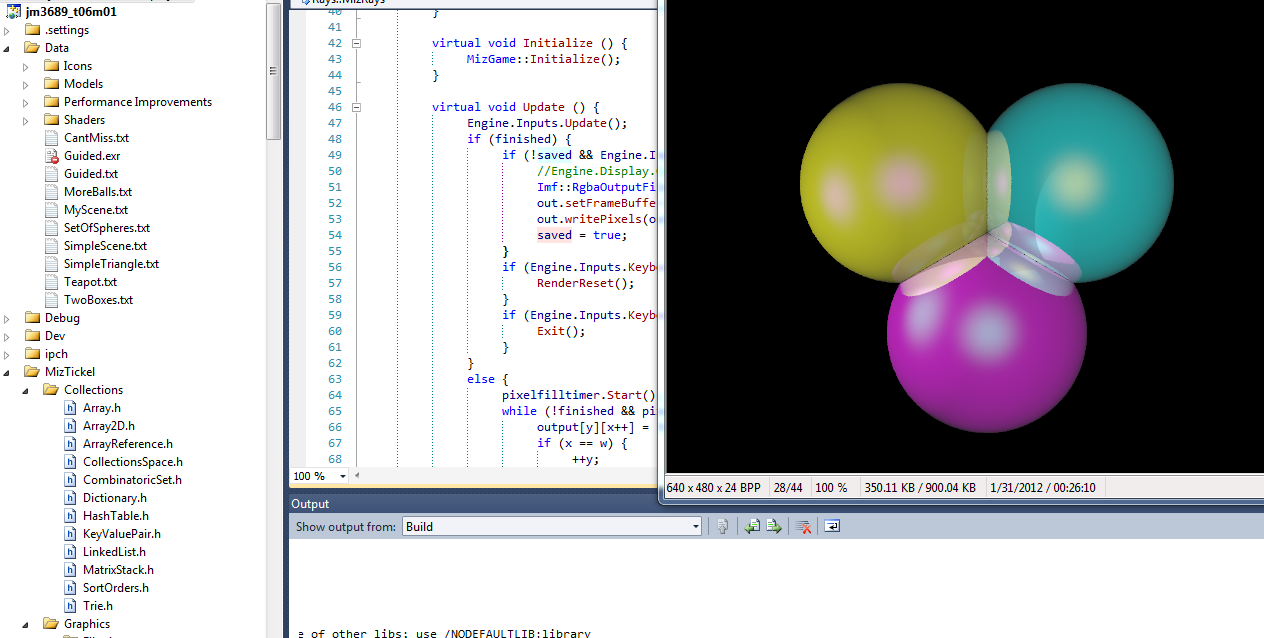
\includegraphics[height=0.4\textheight]{RasterizationsOfFun.png}
  \caption{C++ raytracer; an alternative project. Computes material and shading, along with reflections, for several entities. Developed with \CKey{SDL} and \CKey{OpenGL}.}
  \label{fig:pixelsoffun}
\end{figure}

\begin{figure}
  \centering
  \includegraphics[height=0.4\textheight]{GameDevelopmentBarrelsOfFun.png}
  \caption{Perpixel collision detection in a \textsc{Shootemup} game project, retaining high frames despite using matrices/matrix multiplications and large color maps for the collisions of hundreds (or thousands of entities). Built out of \CKey{C\#} and \CKey{XNA}.}
  \label{fig:gamesoffun}
\end{figure}

For example, building up a Computer Graphics / Ray Tracing engine is titillating pixelated arrays of fun (\figref{pixelsoffun}). Developing a video game engine from scratch would probably make my day as a computer science student (\figref{gamesoffun}). Extending my lexical analyser for OpenGL Shading Language code to do vertex-data-matching based on interleaved array data as a project would be an excellent exercise for the data structures I have created (\figref{lexicalsoffun}). These are only a few small examples on the grand scheme of embedded and non-embedded development; the opportunity not to pick any number of these known projects - or forage into more challenging, more dangerous unknown territory - makes this seem like an opportunity missed to explore true engineering \emph{\textbf{JOY}}.\\

\begin{figure}
  \centering
  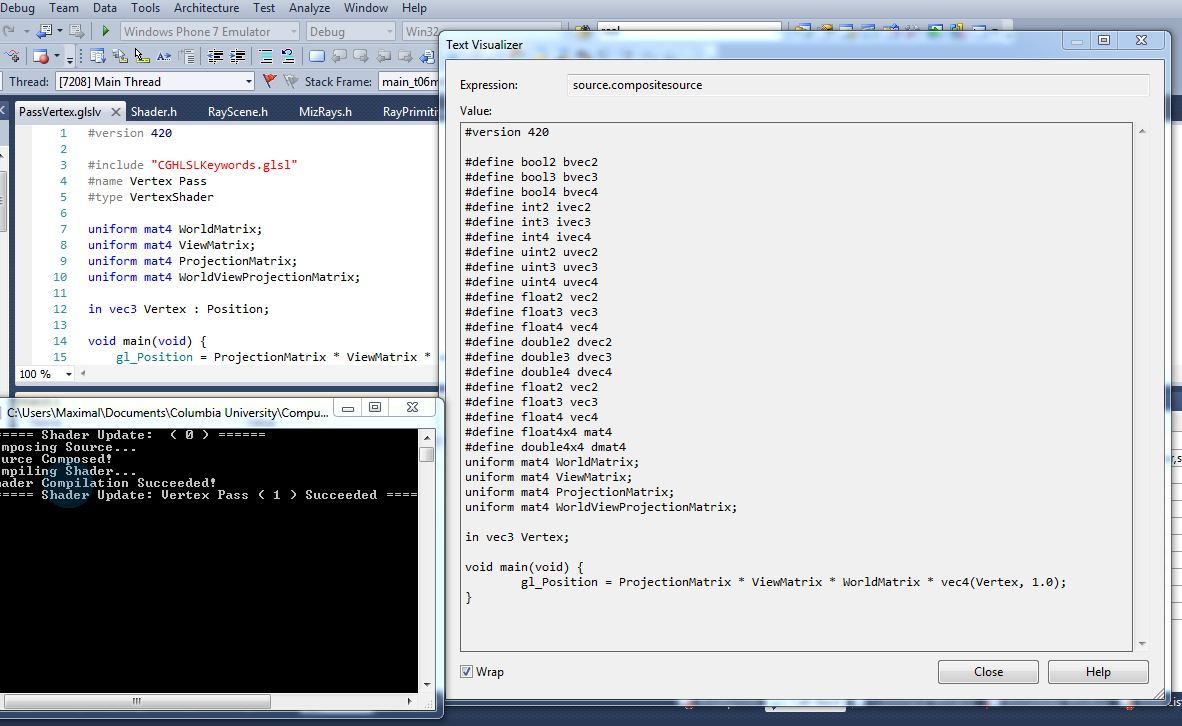
\includegraphics[width=\textwidth]{GLSLShaderLexicalTokenizer.png}
  \caption{A lexical tokenizer for GLSL that takes non-native defines and keywords and parses them, producing GLSL-compatible output code and providing run-time Interleaved Graphics Data type-safety. Developed in \CKey{C++}.}
  \label{fig:lexicalsoffun}
\end{figure}

\section{Source Code}
\label{sec:srccode}
As stated in Section \ref{sec:softdetails}, you can find the source code and an amalgamation of information and build project systems at \url{http://dl.dropbox.com/u/17632594/LibHP20b.tar.gz}. The Linux and Max OSX Makefile may require personal tweaking, especially for the XCode project (Mac OSX does not have any concept of the PATH variable, nor does it use the PATH variable when initializing an external build system).\\

\bibliography{LibHP20b}

\end{document}
